\section{Umsetzung}
Hier werden konkret alle Aspekte der Umsetzung der in \cref{specification} bereits beschriebenen Spezifikation behandelt. %TODO umschreiben
 
\subsection{Initiales Aufsetzen der Anwendung}
Bevor die Entwicklung starten kann müssen die grundlegende Bausteine der Anwendung angelegt, konfiguriert und verbunden werden. 

\subsubsection{Spring Boot Anwendung}\label{spring-boot-init}
Spring stellt eine Weboberfläche zur Verfügung, in der ein komplettes Spring Boot Projekt inklusive Abhängigkeiten einfach generiert werden kann. Die Oberfläche (namens Spring Initializr) erlaubt es Maven oder Gradle als Build-Management-Tool zu verwenden. In diesem Projekt fiel die Entscheidung für Maven, aufgrund der bereits vorhandenen Erfahrung mit dem Tool. 

\begin{figure}[th!]
	\centering
	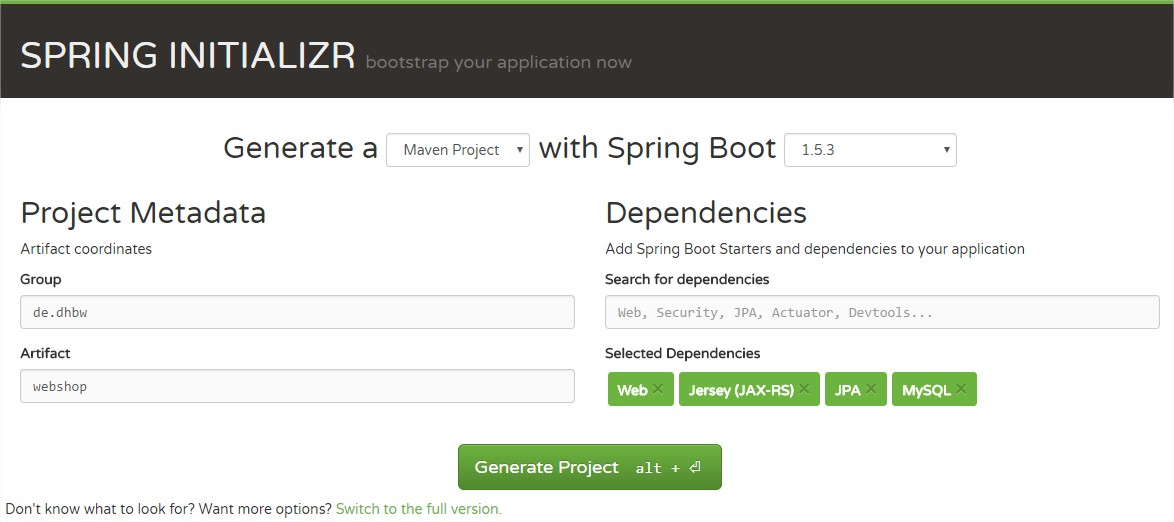
\includegraphics[width=\linewidth]{bilder/kap7/Spring-Initializr}
	\caption{Spring Inititalizr Weboberfläche}
	\label{fig:spring-initializr}
\end{figure}

\cref{fig:spring-initializr} zeigt die gewählte Konfiguration für das Grundprojekt. Links sind die Metadaten für das Deployment definiert und rechts die Abhängigkeiten. Diese sind initial:
\begin{itemize}
	\item \textit{Spring Web}. Benötigt um eine Webanwendung mit eingebetteten Tomcat-Server zu implementieren.
	\item \textit{Jersey}. Hierbei handelt es sich um die Referenzimplementierung von JAX-RS. JAX-RS ermöglicht es, anhand von Annotationen, herkömmliche Java-Klassen per REST verfügbar zu machen. Für die Darstellung dieser Ressourcen verwendet JAX-RS standardmäßig die Implementierung von \acs{JAXB} (Java Architecture for XML Binding). Der Vorteil daran ist, dass die Klassen mit der Annotation \texttt{@XmlRootElement} automatisch bei einem REST Aufruf in die entsprechende XML oder \acs{JSON} Darstellung umgewandelt werden. Die Unterstützung des JSON Formates ist dadurch gewährleistet, dass JAXB die Jackson Bibliotheken benutzt. Die Jackson Bibliothek bietet einen mächtigen Parser für die Konvertierung von Java-Objekten in JSON-Strings\cite{Oracle2015}.
	\item \textit{Spring Data JPA}. Stellt die Zugriffstechnologie der Java Persistence API (\acs{JPA}) zur Verfügung. Mit dieser Abhängigkeit können Datenzugriffsobjekte angelegt werden (sogenannte \acs{DAO}s, Data Access Objects), die alle notwendige Datenbankoperationen implementieren\cite{Webb2017}. 
	\item \textit{Spring MySQL JDBC Driver}. Damit kann die Spring Boot Anwendung automatisch eine Verbindung zur MySQL-Datenbank herstellen\cite{Webb2017}. Alle weitere Konfigurationen für diese Verbindung werden später in \cref{db_umsetzung} beschrieben.
\end{itemize}

Die Ordnerstruktur des generierten Projekts kann der \cref{fig:init-project} entnommen werden. Es handelt sich hierbei um die übliche Struktur einer Java-Anwendung, mit einem \texttt{main} und einem \texttt{test} Verzeichnis. Initial sind im \texttt{main} Verzeichnis nur zwei Dateien: die \texttt{WebshopApplication} Klasse und die \texttt{application.properties}. Erstere enthält die Java \texttt{main}-Methode, welche die Anwendung lauffähig macht. Dort werden auch automatisch alle notwendige Konfigurationen für Spring Boot gesetzt. Die \texttt{application.properties} Datei ist zu diesem Zeitpunkt noch leer, aber sie wird später benutzt um unterschiedliche Aspekte der Anwendung (wie zum Beispiel Server-Port oder Verbindungsdaten zur Datenbank) auf einer einfachen Art und Weise einzustellen.

Eine weitere wichtige Datei ist die \texttt{pom.xml} im Stammverzeichnis. Das Project Object Model oder \acs{POM} ist die grundlegende Arbeitseinheit von Maven. Die XML-Datei enthält Information über das Projekt, sowie Konfigurationsdetails welche von Maven verwendet werden um das Projekt zu bauen. Einige dieser Konfigurationen sind Projekt-Abhängigkeiten, Plugins, Build-Profile usw.\cite{Foundation2017}

\begin{figure}[th!]
	\centering
	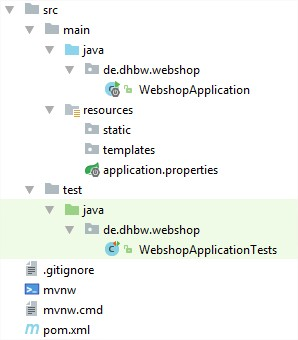
\includegraphics[width=0.5\linewidth]{bilder/kap7/init-project}
	\caption{Ordnerstruktur des generierten Projekts}
	\label{fig:init-project}
\end{figure}

\subsubsection{Angular 2 Anwendung}
Auch hier wird ein Tool eingesetzt, um eine Basisanwendung zu generieren. Hierbei handelt es sich um die Angular CLI, ein Tool für die Initialisierung, Entwicklung und Wartung von Angular Anwendungen\cite{Arora2017}. 

Angular CLI ist ein Open Source Projekt und wird anhand des Node Package Managers (\acs{npm}) installiert. Daraufhin stehen zahlreiche nützliche Befehle für die Kommandozeile zur Verfügung. Für das Generieren einer Angular-Anwendung wird \texttt{ng init} ausgeführt. Der Befehl erstellt alle notwendige Ressourcen, sowie die komplette Konfiguration dazu. Die statische Inhalte werden mit \texttt{ng build} gebaut. 

Damit Spring Boot diese Inhalte verwenden kann müssen sie jedoch im \texttt{resources/static} Verzeichnis liegen. Das kann durch einer Anpassung an der auf \cref{fig:angular-cli} markierten Stelle  der \texttt{angular-cli.json} Datei erreicht werden. Des weiteren enthält diese Datei auch weitere wichtige Konfigurationen, wie der Ablageort von anderen Ressourcen wie Bilder oder benötigte Stylesheets. An dieser Stelle werden demnach die \acs{CSS}-Dateien für das Bootstrap Framework referenziert, sowie eine eigene Stylesheet für weitere Anpassungen. Mehr zu Bootstrap und zu den Designentscheidungen werden später in dieser Arbeit behandelt.

\begin{figure}[th!]
	\centering
	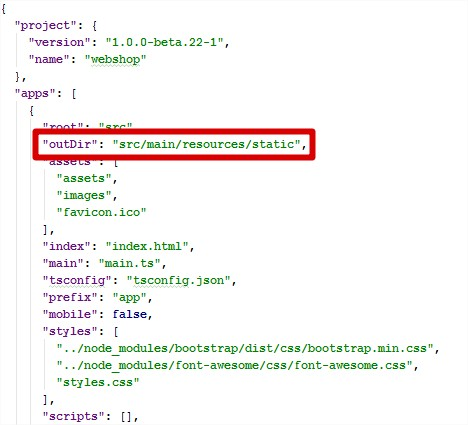
\includegraphics[width=0.8\linewidth]{bilder/kap7/angular-cli}
	\caption{Auszug der Datei angular-cli.json}
	\label{fig:angular-cli}
\end{figure}

\subsection{Backend-Klassen und Objektrelationales Mapping}
%TODO Eine Klasse pro Entität in der Datenbank + DAO-Klasse, Beispiele für die Realisierung von Beziehungen usw. zeigen (ORM-Annotationen)

\subsection{REST-Schnittstellen}
%TODO Aufbau der Rest-Interfaces + Implementierungen, evtl. Klassendiagramme. 

In \cref{spring-boot-init} wurde bereits erwähnt, dass für das Erstellen von REST-Services innerhalb der Spring Boot Anwendung Jersey benutzt wird. Durch die eingebundene Abhängigkeit 

\subsection{Frontend}
%TODO Erstellte Module in Angular 2 (was sind Module? -> Erklären), Struktur von Komponenten, Hauptkomponenten der Module, Services, Routing

\subsubsection{Module}

\subsubsection{Komponenten}

\subsubsection{Services}

\subsubsection{Routing}
